\subsection{CellphoneS}
\begin{figure}[H]
    \centering
    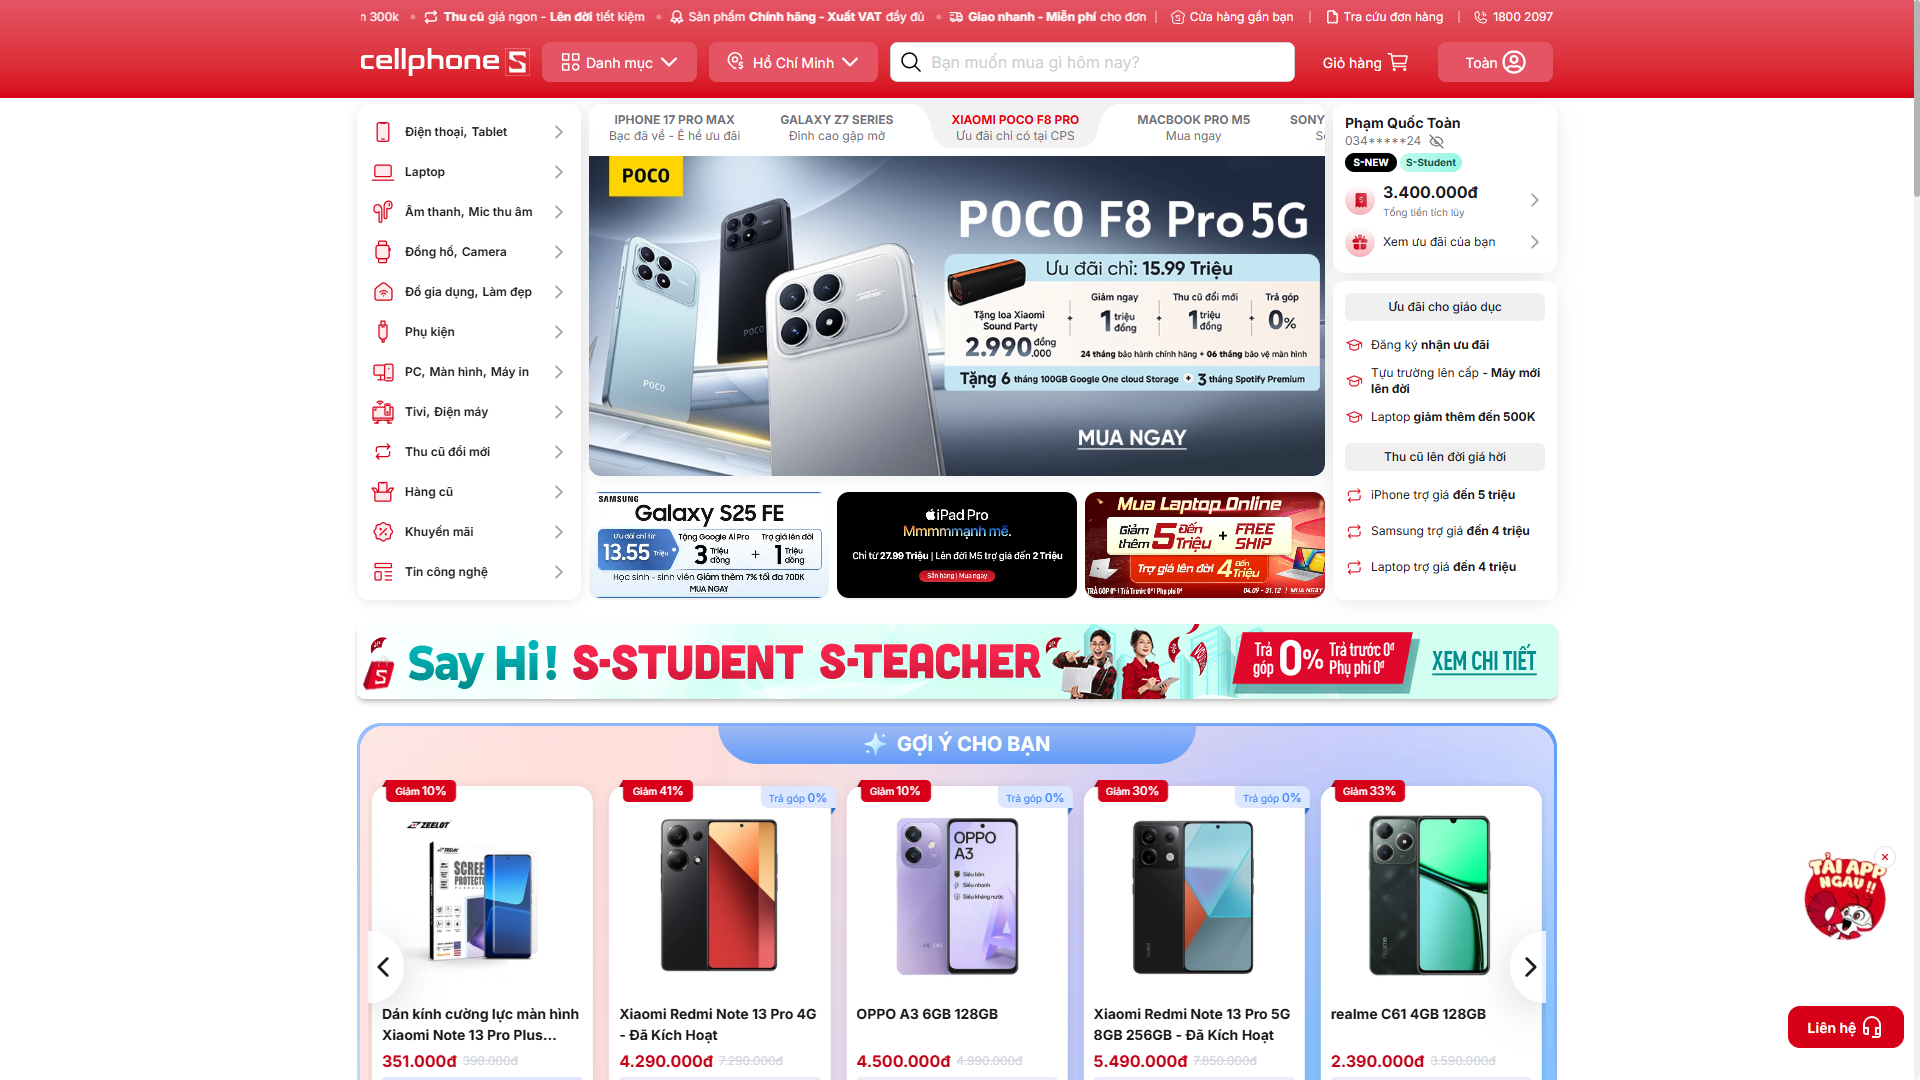
\includegraphics[width=\textwidth]{images/chap2/cellphones.png}
    \vspace{0.5cm}
    \caption{Trang chủ của CellphoneS}
\end{figure}

CellphoneS là hệ thống bán lẻ điện thoại, laptop, máy tính bảng và nhiều phụ kiện công nghệ phổ biến tại Việt Nam, hoạt động song song giữa chuỗi cửa hàng và nền tảng thương mại điện tử. Website của CellphoneS hướng tới trải nghiệm mua sắm nhanh, tiện lợi, hỗ trợ trả góp, chương trình thu cũ đổi mới (trade-in) và hệ thống tích điểm khách hàng thân thiết Smember.

\textbf{Tính năng nổi bật:}
\begin{itemize}
    \item Bộ lọc và tìm kiếm sản phẩm theo giá, thương hiệu, thông số kỹ thuật và chương trình khuyến mãi.
    \item Hỗ trợ trade-in với quy trình định giá trực tuyến và phản hồi nhanh.
    \item Trả góp linh hoạt qua nhiều hình thức như thẻ tín dụng, công ty tài chính hoặc ví điện tử.
    \item Ứng dụng Smember giúp người dùng quản lý điểm thưởng, theo dõi ưu đãi và thông báo khuyến mãi.
\end{itemize}

Website của CellphoneS thể hiện thế mạnh rõ rệt ở việc xây dựng quy trình trade-in minh bạch và dễ sử dụng, cùng với hệ thống trả góp linh hoạt, giúp người dùng có nhiều lựa chọn tài chính phù hợp. Nền tảng Smember tạo ra hệ sinh thái khách hàng thân thiết, góp phần giữ chân người dùng lâu dài. Tuy nhiên, website vẫn còn hạn chế ở khả năng cá nhân hóa trải nghiệm mua sắm. Các tính năng như đề xuất sản phẩm thông minh hay chatbot hỗ trợ tương tác tự nhiên chưa được đầu tư sâu, khiến hệ thống vẫn chủ yếu hoạt động theo cơ chế tìm kiếm và thao tác thủ công.
